\chapter{Anhang}

\section{Prozesseübersicht Unternehmensebene} \label{sec:AnhangA1}

\begin{figure}
    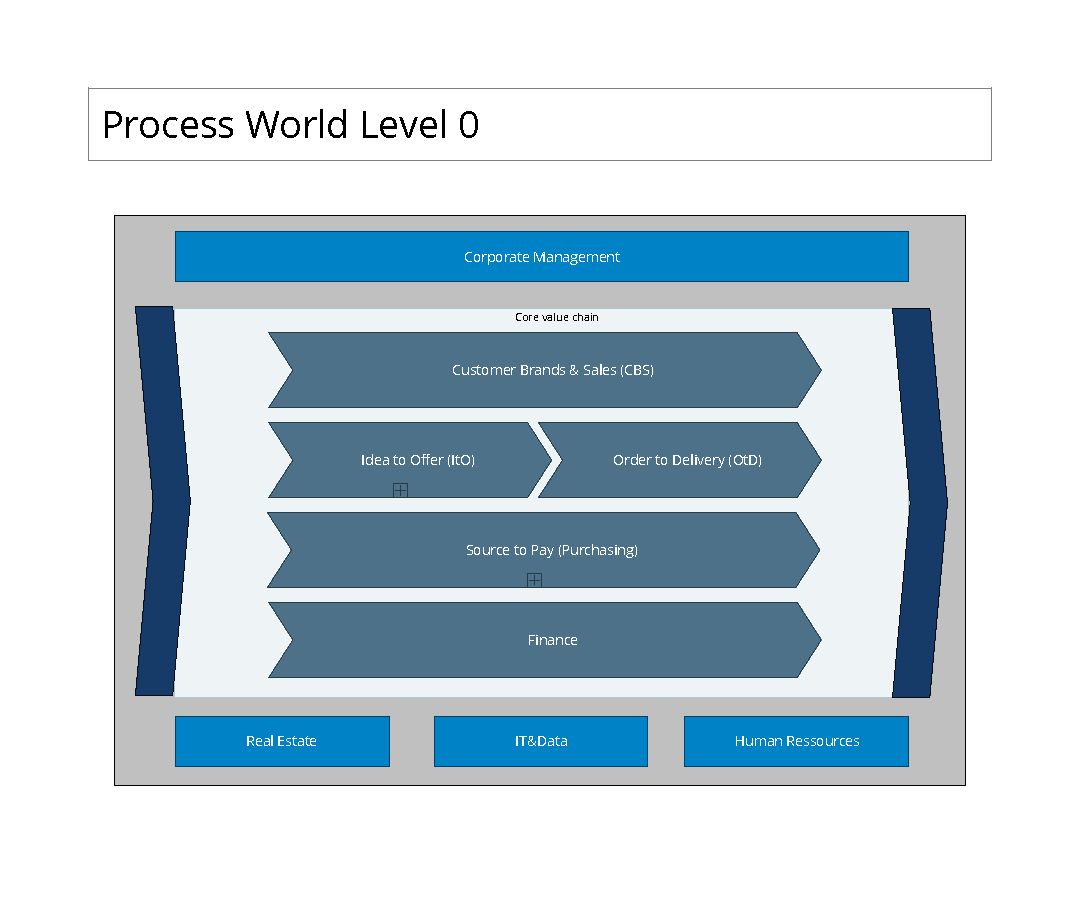
\includepdf[]{Inhalt/Literatur/Process_World_Level_0.pdf}
\end{figure}
\clearpage

\section{Prozessübersicht Source-to-Pay} \label{sec:AnhangA2}

\begin{figure}
    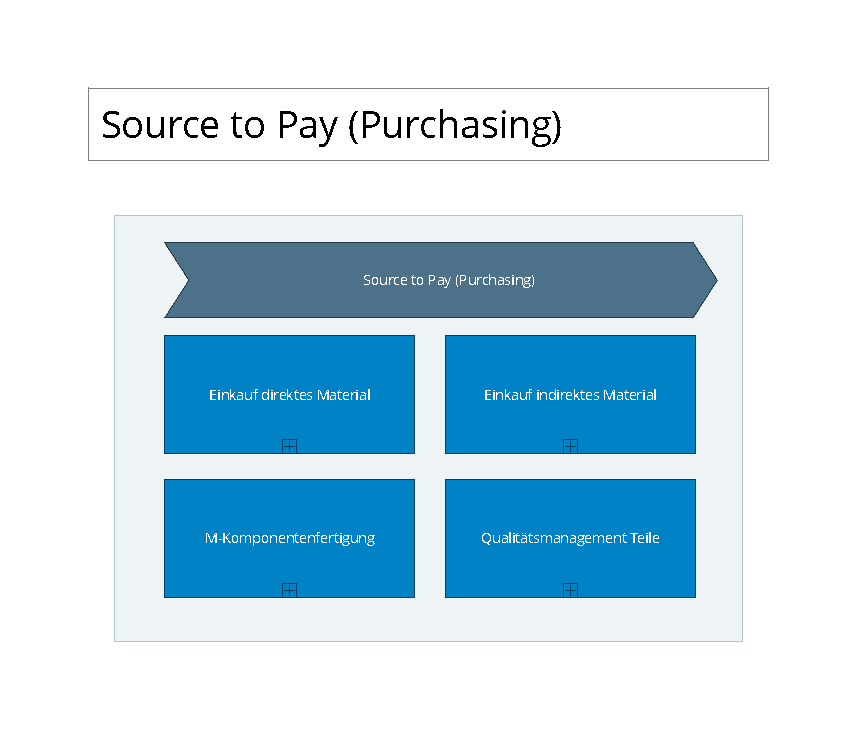
\includepdf[]{Inhalt/Literatur/Source_to_Pay.pdf}
\end{figure}
\clearpage

\section{Prozessübersicht Einkauf direktes Material} \label{sec:AnhangA3}

\begin{figure}
    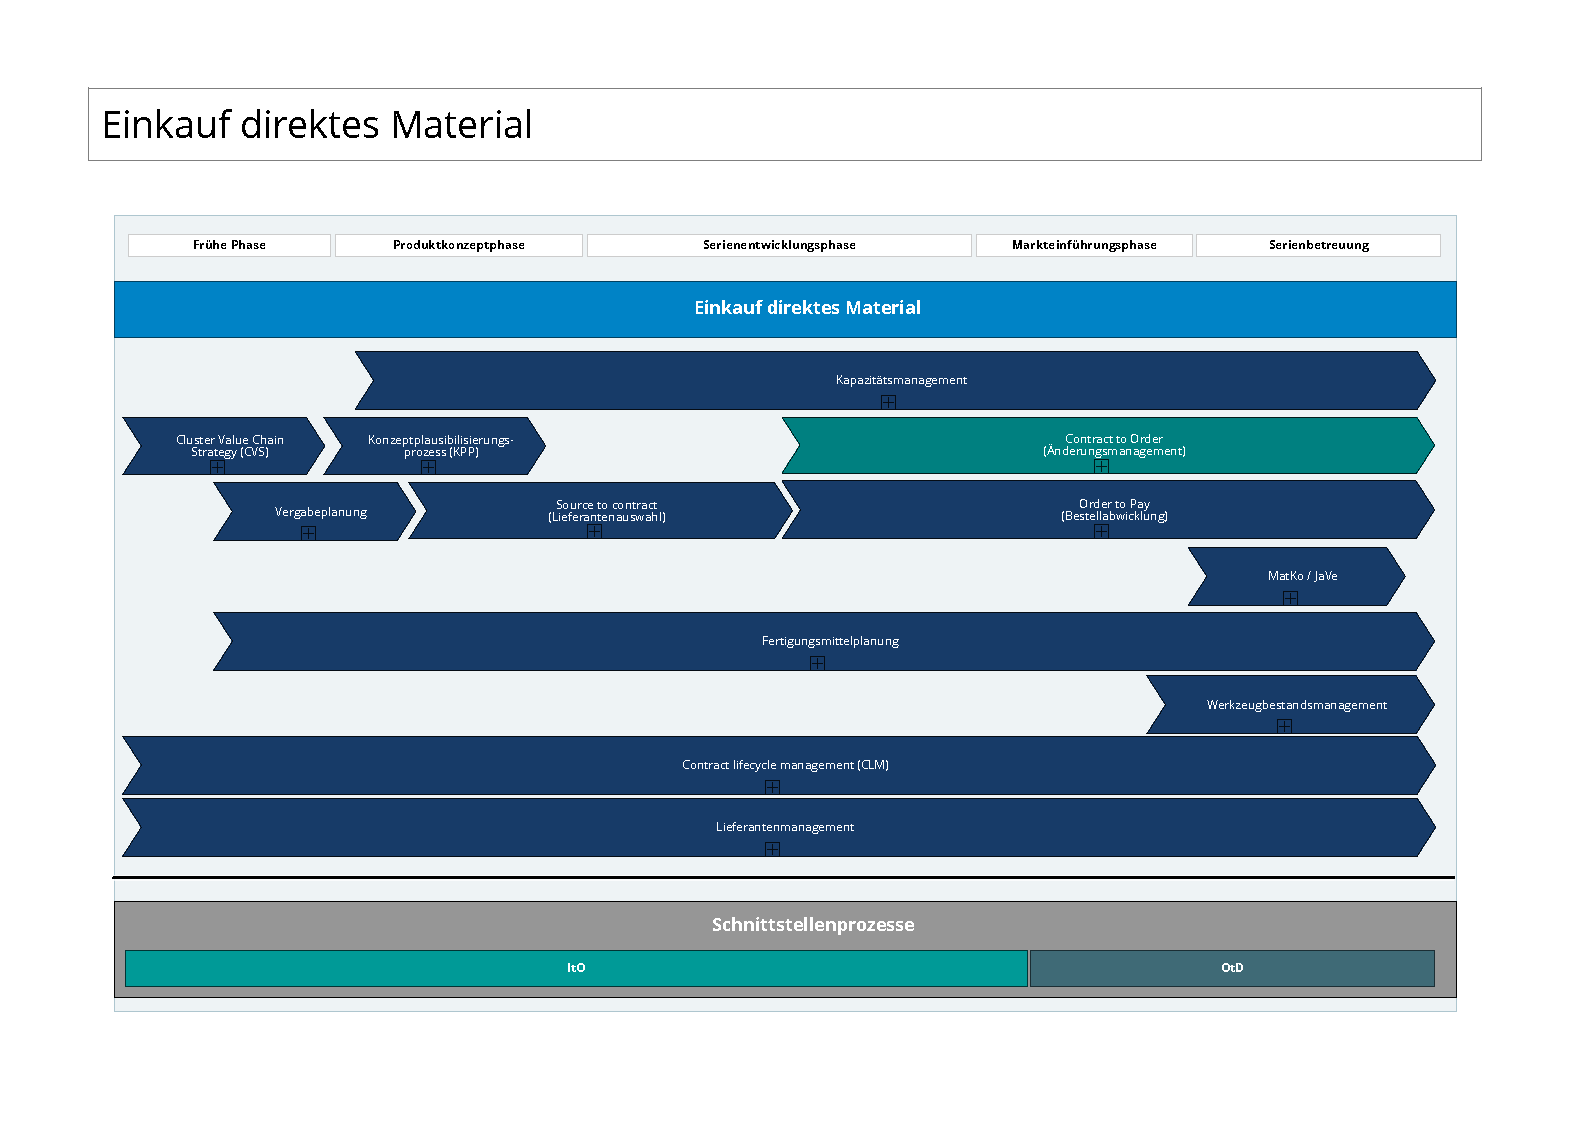
\includepdf[angle = 90, fitpaper = true]{Inhalt/Literatur/Einkauf_direktes_Material.pdf}
\end{figure}
\clearpage

\section{Transkript Expterteninterview Anforderungen an neuen Prozess}

\textbf{Befragender:} Tom Wolfrum (Abkürzung: \textbf{T})

\textbf{Befragter:} Georg Bandouch, \textit{Projektmanager Global Sourcing System and Procurement Process Redesign} (Abkürzung: \textbf{G})

\textbf{Datum:} 15.06.2024

\begin{list}{X:}{\setlength{\labelsep}{5mm}}
 \linenumbers[1]
 \item[\textbf{T}:] Hallo Georg, vielen Dank, dass du dir die Zeit für dieses Interview im Rahmen meiner Praxisarbeit genommen hast. Zuerst aber eine formale Frage: Ich würde dieses Interview aufzeichnen und im Anschluss transkribieren, um es dann für meine Praxisarbeit zu verwenden. Bist du damit einverstanden?
 \item[\textbf{G}:] Hallo Tom, ja bin ich.
 \item[\textbf{T}:] Super, dann lass und gleich loslegen. Thematisch soll es heute ja um die Anforderungen an den neuen Prozess zur Massenbearbeitung der Central Contracts gehen. Doch starten wir bei dir als Person. Wer bist du und was ist deine Aufgabe im Unternehmen? Du kannst auch darauf eingehen, inwiefern du mit Central Contracts bzw. deren Massenbearbeitung in Kontakt kommst.
 \item[\textbf{G}:] Ich arbeite als Projektmanager im Bereich Global Sourcing System und Procurement Process Redesign bei BMW. In dieser Funktion bin ich auf der einen Seite für den operativen Betrieb unserer IT-Systeme im Einkauf zuständig und auf der anderen Seite für die kontinuierliche Weiterentwicklung unserer Beschaffungsprozesse. Aktuell bin ich noch sehr viel mit der Betreuung unseres SAP-Altsystems SRM beschäftigt, das wir in den nächsten Jahren durch die neue S/4-Suite \footnote{Gemeint ist hier ''SAP Ariba Direct Materials Sourcing for Automotive and Industrial Manufacturing in SAP S/4 HANA''} ablösen wollen. Da ich diese Systeme im Produktivbetrieb dann auch betreuen muss,  bin ich natürlich auch in diesem gro\ss en Implementierungsprojekt stark involviert. Insgesamt bin ich aber eher auf der IT- als auf der Business-Seite zu finden.
 \item[\textbf{T}:] Wie genau kommst du hier mit Central Contracts bzw. deren Massenbearbeitung in Kontakt?
 \item[\textbf{B}:] Zentralkontrakte sind für uns im Einkauf schon immer ein wichtiges Thema gewesen. Wir müssen, nachdem mit einem Lieferanten eine Einigung erzielt wurde, dass er uns ein Bauteil über die nächsten Jahre hinweg in bestimmten Mengen zu einem bestimmten Preis beliefert, diese Übereinkunft auch im System abbilden können. Ich meine hier nicht den rechtlichen Vertrag, darum kümmern sich andere Abteilungen in eigenen Systemen, sondern den Vertrag als Objekt, den wir dann an die lokalen Werkssysteme in den einzelnen Standorten verteilen. Und dieser Vertrag dient den lokalen Werken dann als Bestellgrundlage, da die mit den Lieferanten vereinbarten Mengen ja nur Abrufbudgets sind aus denen wir dann unsere tatsächlichen Bedarfe abrufen. Das sollen dann in der Zukunft die Central Contracts übernehmen.
 \item[\textbf{T}:] Und wie sieht es mit der Massenbearbeitung aus?
 \item[\textbf{G}:] Die Massenbearbeitung ist für uns essentiell wichtig, damit die Facheinkäufer auch das neue System akzeptieren und benutzen. Wir haben tausende Verträge, die wir alle mindestens einmal im Jahr im Rahmen der JaVe \footnote{Gemeint ist die Jahrespreisverhandlung} anpassen müssen. Das hei\ss t, jeder Facheinkäufer muss die Änderungen, die er mit dem Lieferanten ausgehandelt hat, ins System einpflegen. Das können neue Preise, Konditionen oder Zuschläge sein. Und alle diese Daten haben noch Gültigkeitszeiträume. Wenn man neben der gro\ss en Anzahl an Verträgen auch die ca. 400 verschiedenen Konditionen bedenkt, kann man sich denken, dass manche Facheinkäufer da sehr lange dran sitzen. Deshalb ist es für uns so wichtig, dass wir für die Massenbearbeitung einen effizienten Prozess haben, den die Facheinkäufer verstehen. Wenn sie Fehler machen, bin ich nämlich derjenige, der das dann im System wieder nacharbeiten muss.
 \item[\textbf{T}:] Ok, das unterstreicht auf jeden Fall nochmal die Dringlichkeit, dass wir hier eine Lösung finden. Lass und mal zu den Anforderungen an einen neuen Prozess kommen. Was ist aus deiner Sicht hier besonders wichtig, also welche Anforderungen muss der neue Prozess unbedingt erfüllen?
 \item[\textbf{G}:] Ich denke der Oberbegriff ist die User Experience. Die ist aktuell im Prozess, so wie ihr \footnote{Gemeint ist die SAP SE im Allgemeinen, bezogen auf die Massenbearbeitungsfunktionalität von Central Contracts im Standard} den im Standard ausliefert und wie wir ihn aktuell verwenden, für unsere Situation einfach nicht gut. Klar, für viele einfache Felder im Central Centract reicht uns die Online-Massenpflege aus dem Standard. Wenn wir einfach nur bei vielen Kontrakten ein bestimmtes Feld mit einem Wert überschreiben müssen, funktioniert das gut. Für mich wichtig sind aber vor allem die Basispreise, Konditionen, Rohstoffe und deren Gültigkeitszeiträume. Hier müssen nämlich bei jedem Vertrag andere Änderungen gemacht werden, womit das Online-Feature schonmal rausfällt, egal ob man hier etwas Customizen könnte oder nicht. Dann bleibt uns noch die Pflege per Excel. Das ist aber für uns in der aktuellen Variante absolut ungeeignet. Es hat sehr viele Felder, von denen die meisten für uns garnicht relevant sind und die Struktur der Tabs ist sehr unübersichtlich. Allgemein ist das Excel einfach so überladen, dass die Facheinkäufer aktuell viel zu viele Fehler machen. Allgmein sollte ich vielleicht noch dazusagen, dass der Basispreis immer die Basis für alle weiteren Konditionen, Rohstoffe und Zuschläge, etc. bildet. Das hei\ss t, wir haben immer einen Basispreis, auf den dann verschiedene Konditionen, Rohstoffe und Zuschläge aufgeschlagen werden.
 \item[\textbf{T}:] Ich habe herausgehört, das für dich vorallen Basispreiseintervalle, Konditionen und Rohstoffe wichtig sind. Kannst du mir genauer erklären, welche Anforderungen du in diesem Bereich hast?
 \item[\textbf{G}:] Klar. Ein Punkt ist die rückwirkende Massenänderung. Die JaVe findet bei uns meist für ein Jahr X im Sommer diesen Jahres statt. Das hei\ss t die Massenänderungen müssen auch rückwirkend möglich sein, da ein Facheinkäufer \zB im August die Preise für den vergangen Januar verhandeln könnte. Eine weitere Anforderung betrifft die Zeitintervalle. Im Vertrag gibt es ja schon vor der JaVe über die komplette Belieferungsdauer eines Teils fertig gepflegte Basispreise, Konditionen, etc. mit ihren jeweiligen Gültigkeitsintervallen. Von diesen müssen wir beliebig abweichen können. Das hei\ss t konkret: Betrachten wir hypothetisch ein hypothetisches Jahr. Aktuell haben wir hier vier Basispreisintervalle mit verschiedenen Werten anhand der Quartale des Jahres. Wenn der Facheinkäufert jetzt mit dem Lieferanten aushandelt, dass vom 15.02. bis zum 31.05. ein neuer Basispreis gilt, passt dieser zu keinem der bestehenden Intervalle. Aktuell müsste er hingehen, das erste Intervall (also Q1) am Ende verkürzen und das zweite Intervall (also Q2) später beginnen lassen, um Platz für das neue Intervall zu schaffen. Hier wäre es gut, wenn das System diese Intervalle automatisch anpassen könnte, wenn der Einkäufer etwas einfügt. Einen wichtigen Sonderfall gibt es noch: Wir verwenden für internationale Lieferanten teilweise Fremdwährungszuschläge. Diese müssen wir aus bilanz-technischen Gründen immer quartalsweise berechnen. Das hei\ss t, wenn so ein Zuschlag einem Basispreisintervall hinzugefügt wird muss dieses Intervall immer an den Quartalsgrenzen einmal geteilt werden und danach ggf. als neues Intervall weitergehen. Das ist aktuell sehr aufwändig und fehleranfällig, wenn ein Facheinkäufer das nacharbeiten muss. Eine Einschäkung gibt es noch bei der rückwirkenden Massenänderung: Die Facheinkäufer sollen maximal zwölf Monate rückwirkend Änderungen machen können. Die Ausnahme sind bestimmte User, wie ich und meine Kollegen, die die Systeme auch administrativ betreuen. Wir müssten schon bis zu 36 Monaten in der Vergangenheit noch Änderungen machen können.
 \item[\textbf{T}:] Du bist jetzt speziell auf rückwirkende Änderungen eingegangen, ist das der einzige Fall, oder gibt es auch noch andere Fälle der Massenänderung?
 \item[\textbf{G}:] Nein, das ist nicht der einzige Fall. Es kommt auch vor, das wir für die Zukunft planen und verhandeln müssen. Das hei\ss t, es müssen auch Intervalle, die noch in der Zukunft liegen angepasst werden können. Hier ist wichtig, dass wir keine ''Lücken'' zwischen unseren Basispreisintervallen haben dürfen. Das hei\ss t, wenn ein Facheinkäufer ein neues Intervall einfügen würde, das keinen direkten Vorgänger hätte, müsste das zeitlich gesehen letzte vorherige Intervall bis zum Beginn des eingefügten Intervalls verlängert werden. Ich versuche das vielleicht nochmal an einem Beispiel deutlich zu machen: Angenommen es wird ein Intervall vom 01.01.2024 bis zum 31.03.2024 eines Jahres eingefügt und das letzte vorherige Intervall endet aber schon am 30.09.2023 des Vorjahres. Das hei\ss t, wir hätten eine Lücke von drei Monaten zwischen den beiden Intervallen. Das darf nicht passieren, deshalb müsste das letzte Intervall bis zum 31.12.2023 verlängert werden.
 \item[\textbf{T}:] Danke für die Klarstellung, ich denke ich habe den Anwendungsfall gut verstanden. Gibt es auch Anforderungen, die nicht im Bezug auf Gültigkeitszeiträume bestehen?
 \item[\textbf{G}:] Wenn wir rein von einer Anpassung von Werten sprechen, ohne Gültigkeitszeiträume zu veränderung müssen wir eigentlich relativ wenig beachten. Klar dürfen nur sinnvolle Werte eingegeben werden, wie \zB ein negativer Basispreis ergibt zum Beispiel keinen Sinn, aber das ist ja kein Thema, das nur speziell für die Massenpflege gilt. Genrell soll es ja so sein, dass das, was der Facheinkäufer über die Massenänderung ins System eingibt, immer die vorhandenen Daten im jeweiligen Gültigkeitszeitraum überschreiben soll.
 \item[\textbf{T}:] Du hast am Anfang noch davon gesprochen, dass die aktuelle Excel-Lösung für euch nicht geeignet und sehr unübersichtlich ist. Kannst du das weiter ausführen?
 \item[\textbf{G}:] Was ich damit gemeint habe ist einerseits, dass wir für die Massenbearbeitung nur zwei der insgesamt acht Tabs des Tabelle benötigen. Auf den Reitern, die wir tatsächlich bearbeiten wollen sind dann noch sehr viele Felder enthalten, die für uns nicht relevant sind. Generell ist aber einfach zu viel auf einmal anpassbar: Verschiedene Verträge, Vertrags-Items, Gültigkeitszeiträume, Konditionen, Werte und so weiter. Es wäre für die User Experience sehr vorteilhaft, wenn man die Massenpflege in mehrere Schritte aufteilen könnte, sodass der Einkäufer sich nicht um alles auf einmal Gedanken machen muss. 
 \item[\textbf{T}:] Wie sieht es mit einer Prüflogik aus, müssen Ergebnisse validiert werden?
 \item[\textbf{G}:] Wir benötigen auf jeden Fall eine Simulation und Validierung der Ergebnisse, bevor diese final in das System übernommen werden. Wenn der Einkäufer einen Fehler macht, muss er diesen angezeigt bekommen und korrigieren können. 
 \item[\textbf{T}:] Fallen dir sonst noch weitere Anforderungen an den neuen Prozess bzw. die Lösung ein?
 \item[\textbf{G}:] Nein, ich glaube, das wäre es erstmal.
 \item[\textbf{T}:] Dann bedanke ich mich für deine Zeit und das Interview. Die Anforderungen werden mir sehr helfen, ein passendes Konzept für den neuen Prozess auszuarbeiten. Das Interview werde ich im Anschluss noch transkribieren und dir zur Freigabe zukommen lassen.
 \item[\textbf{G}:] Hört sich gut an, ich bin gespannt auf die Ergebnisse. Vielen Dank und bis bald.
 \item[\textbf{T}:] Ich habe zu danken. Auf Wiedersehen.     
\end{list}